
\chapter{Simple Derivatives}

A derivative with respect to a tensor is simply the collection of derivatives with respect to each element of this tensor.
We can keep track of $\frac{d T}{d U}$ by making a tensor of shape $\mathrm{shape}(T) \cup \mathrm{shape}(U)$.
For example, if $T$ is an order-3 tensor and $U$ is an order-2 tensor, we draw $dT/dU$ as
\[
   \frac{dT}{dU} =
   \vcenter{\hbox{
      \import{figures/}{dTdU.pdf_tex}
   }}
\]
This notation follows Penrose.
The two extra lines coming from the black dot on the circle makes the derivative an order-5 tensor.
That the order of derivatives grows this way, is one of the main reasons we'll encounter for tensors to show up in the first place.

When there are not too many edges, we will use a simple inline notation like this:
\[
\begin{tikzpicture}[baseline=(T.base), inner sep=1pt]
   \node (T) {$(T)$};
   \draw (T) -- ++(-.5,-.1);
   \draw (T) -- ++(-.5,+.1);
   \draw (T) -- ++(+.5,0);
   \draw[d] (T.east) -- ++(.2,.2);
   \draw[d] (T.east) -- ++(.3,.1);
\end{tikzpicture}
\]

The Matrix Cookbook defines the single-entry matrix $J^{i,j} \in R^{n\times n}$ as the matrix which is zero everywhere except in the entry $(i, j)$ in which it is 1.
Alternatively we could write $J^{i,j}_{n,m} = [i=n][j=m]$.

\section{Derivatives of Matrices, Vectors and Scalar Forms}

\subsection{First Order}
The following first order derivatives show the basic linearity properties of the derivative operator.

\begin{walign}
   \tag{69}
   \frac{\partial x^T a}{\partial x}
   &= a
   &
      \begin{tikzpicture}[baseline=(a0.base), inner sep=1pt]
         \node (a0) {$(x$};
         \node[right=1em of a0] (a1) {$a)$};
         \path (a0) edge (a1);
         \draw [d] (a1.east) -- ++(-.2,.2);
      \end{tikzpicture}
   &=
      \begin{tikzpicture}[baseline=(a0.base), inner sep=1pt]
         \node (a0) {$(x)$};
         \node[right=1em of a0] (a1) {$a$};
         \path (a0) edge (a1);
         \draw [d] (a0.east) -- ++(-.2,.2);
      \end{tikzpicture}
   =
      \begin{tikzpicture}[baseline=(a.base), inner sep=1pt]
         \draw (0,0) node[right] (a) {$a$} -- ++(-.3, 0);
      \end{tikzpicture}
   \\
   %%%%%%%%%%%%%%%%%%%%%%%%%%%%%%%%%%%%%%%%
   \tag{69}
   \frac{\partial a^T x}{\partial x}
   &= a
   &
      \begin{tikzpicture}[baseline=(a0.base), inner sep=1pt]
         \node (a0) {$(a$};
         \node[right=1em of a0] (a1) {$x)$};
         \path (a0) edge (a1);
         \draw [d] (a1.east) -- ++(-.2,.2);
      \end{tikzpicture}
   &=
      \begin{tikzpicture}[baseline=(a0.base), inner sep=1pt]
         \node (a0) {$(x)$};
         \node[left=1em of a0] (a1) {$a$};
         \path (a0) edge (a1);
         \draw [d] (a0.east) -- ++(-.2,.2);
      \end{tikzpicture}
   =
      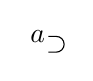
\begin{tikzpicture}[baseline=(a.base), inner sep=1pt]
         \node (a) {$a$};
         \draw (a.east) -- ++(.1, 0) arc (270:90:-.1) -- ++(-.1, 0);
      \end{tikzpicture}
   =
      \begin{tikzpicture}[baseline=(a.base), inner sep=1pt]
         \draw (0,0) node[right] (a) {$a$} -- ++(-.3, 0);
      \end{tikzpicture}
   \\
   %%%%%%%%%%%%%%%%%%%%%%%%%%%%%%%%%%%%%%%%
   \tag{70}
   \frac{\partial a^T X b}{\partial X} &= ab^T
   &
      \begin{tikzpicture}[baseline=(a0.base), inner sep=1pt]
         \node (a0) {$(a$};
         \node[right=1em of a0] (a1) {$X$};
         \node[right=1em of a1] (a2) {$b)$};
         \path (a0) edge (a1);
         \path (a1) edge (a2);
         \draw[d] (a2.east) -- ++(.2,.2);
         \draw[d] (a2.east) -- ++(.3,.1);
      \end{tikzpicture}
   &=
      \begin{tikzpicture}[baseline=(a0.base), inner sep=1pt]
         \node (a0) {$a$};
         \node[right=1em of a0] (a1) {$(X)$};
         \node[right=1em of a1] (a2) {$b$};
         \path (a0) edge (a1);
         \path (a1) edge (a2);
         \draw[d] (a1.east) -- ++(.2,.2);
         \draw[d] (a1.east) -- ++(.3,.1);
      \end{tikzpicture}
      =
      \begin{tikzpicture}[baseline=(a.base), inner sep=1pt]
         \node (a) {$a$};
         \draw (a) -- ++(.3, 0) arc (270:90:-.1);
         \node[right=2em of a] (b) {$b$};
         \draw (b) -- ++(-.3, 0) arc (270:90:.1);
      \end{tikzpicture}
   \\
   %%%%%%%%%%%%%%%%%%%%%%%%%%%%%%%%%%%%%%%%
   \tag{73}
   \frac{\partial X}{\partial X_{i,j}} &= J^{i,j}
   &
      \begin{tikzpicture}[baseline=(a0.base), inner sep=1pt]
         \node (a0) {$($};
         \node[right=1em of a0] (a1) {$X$};
         \node[right=1em of a1] (a2) {$)$};
         \draw (a0) -- (a1) -- (a2);
         \draw[d] (a2.east) -- ++(.2,.2) node[midway, above left, font=\tiny] {i};
         \draw[d] (a2.east) -- ++(.3,.1) node[midway, below right, font=\tiny] {j};
      \end{tikzpicture}
   &=
      \begin{tikzpicture}[baseline=(a.base), inner sep=1pt]
         \node (a) {};
         \draw (a) -- ++(.3, 0) arc (270:90:-.1) node[pos=1, below left, font=\tiny] {i};
         \node[right=2em of a] (b) {};
         \draw (b) -- ++(-.3, 0) arc (270:90:.1) node[pos=1, above right, font=\tiny] {j};
      \end{tikzpicture}
   \\
   %%%%%%%%%%%%%%%%%%%%%%%%%%%%%%%%%%%%%%%%
   \tag{74}
   \frac{\partial (X A)_{i,j}}{\partial X_{m,n}} &= (J^{m,n} A)_{i,j}
   &
      \begin{tikzpicture}[baseline=(a0.base), inner sep=1pt]
         \node (a0) {$($};
         \node[right=1em of a0] (a1) {$X$};
         \node[right=1em of a1] (a2) {$A$};
         \node[right=1em of a2] (a3) {$)$};
         \draw (a0) -- (a1) node[midway, above left, font=\tiny] {i};
         \draw (a1) -- (a2);
         \draw (a2) -- (a3) node[midway, below right, font=\tiny] {j};
         \draw[d] (a3.east) -- ++(.2,.2) node[midway, above left, font=\tiny] {m};
         \draw[d] (a3.east) -- ++(.3,.1) node[midway, below right, font=\tiny] {n};
      \end{tikzpicture}
   &=
      \begin{tikzpicture}[baseline=(a0.base), inner sep=1pt]
         \node (a0) {};
         \node[right=1em of a0] (a1) {$(X)$};
         \node[right=1em of a1] (a2) {$A$};
         \node[right=1em of a2] (a3) {};
         \path (a0) edge (a1);
         \path (a1) edge (a2);
         \path (a2) edge (a3);
         \draw[d] (a1.east) -- ++(.2,.2);
         \draw[d] (a1.east) -- ++(.3,.1);
      \end{tikzpicture}
 \\&&&=
      \begin{tikzpicture}[baseline=(a0.base), inner sep=1pt]
         \node (a0) {};
         \node[right=1em of a0] (a1) {};
         \node[right=1em of a1] (a2) {$A$};
         \node[right=1em of a2] (a3) {};
         \draw (a0) -- (a1) node[midway, above left, font=\tiny] {i};
         \draw (a1) -- (a2);
         \draw (a2) -- (a3) node[midway, below right, font=\tiny] {j};
         \draw (a1.west) -- ++(.1,.2) node[midway, above left, font=\tiny] {m};
         \draw (a1.east) -- ++(-.1,-.2) node[midway, below right, font=\tiny] {n};
      \end{tikzpicture}
\end{walign}

\subsection{Second Order}
The second order derivatives are follow from the product rule:
\[
   \vcenter{\hbox{
      \import{figures/}{product.pdf_tex}
   }}
\]
Note that this rule holds independently of how many edges are between $T$ and $U$, even if there are none.

\begin{walign}
   \tag{76}
   \frac{\partial}{\partial X_{i,j}}
   \sum_{k,l,m,n} X_{k,l} X_{m,n}
   &= (\sum_{k,l} X_{k,l})^2
   %&= \frac{\partial \|X\|_F^2}{\partial X_{i,j}}
   %&= 2\, \sum_{k,l} X_{k,l}
   &
   \begin{tikzpicture}[baseline=.5em, inner sep=1pt]
      \node (a0) at (0,0) {$\sbullet$};
      \node (a1) at (.5,0) {$X$};
      \node (a2) at (1,0) {$\sbullet$};
      \path (a0) edge (a1);
      \path (a1) edge (a2);
      \node (b0) at (0, .5) {$\sbullet$};
      \node (b1) at (.5, .5) {$X$};
      \node (b2) at (1, .5) {$\sbullet$};
      \path (b0) edge (b1);
      \path (b1) edge (b2);
      \node at (-.25, .25) {$\bigg($};
      \node at (1.25, .25) {$\bigg)$};
      \draw[d] (1.35, .4) -- ++(.2,.2) node[midway, above left, font=\tiny] {i};
      \draw[d] (1.35, .4) -- ++(.3,.1) node[midway, below right, font=\tiny] {j};
   \end{tikzpicture}
   &=
   \begin{tikzpicture}[baseline=.5em, inner sep=1pt]
      \node (a0) at (0,0) {$\sbullet$};
      \node (a1) at (.5,0) {$(X)$};
      \node (a2) at (1,0) {$\sbullet$};
      \path (a0) edge (a1);
      \path (a1) edge (a2);
      \node (b0) at (0, .5) {$\sbullet$};
      \node (b1) at (.5, .5) {$X$};
      \node (b2) at (1, .5) {$\sbullet$};
      \path (b0) edge (b1);
      \path (b1) edge (b2);
      \draw[d] (.83,.0) -- ++(.2,.2);
      \draw[d] (.83,.0) -- ++(.3,.1);
   \end{tikzpicture}
   +
   \begin{tikzpicture}[baseline=.5em, inner sep=1pt]
      \node (a0) at (0,0) {$\sbullet$};
      \node (a1) at (.5,0) {$X$};
      \node (a2) at (1,0) {$\sbullet$};
      \path (a0) edge (a1);
      \path (a1) edge (a2);
      \node (b0) at (0, .5) {$\sbullet$};
      \node (b1) at (.5, .5) {$(X)$};
      \node (b2) at (1, .5) {$\sbullet$};
      \path (b0) edge (b1);
      \path (b1) edge (b2);
      \draw[d] (0.83,.5) -- ++(.2,.2);
      \draw[d] (0.83,.5) -- ++(.3,.1);
   \end{tikzpicture}
   %\\[.3em]
   \\
   &= 2\, \sum_{k,l} X_{k,l}
   &&=
   2\,
   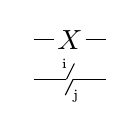
\begin{tikzpicture}[baseline=.5em, inner sep=1pt]
      \node (a0) at (0,0) {$\sbullet$};
      \node (a1) at (.5,0) {};
      \node (a2) at (1,0) {$\sbullet$};
      \path (a0) edge (a1);
      \path (a1) edge (a2);
      \node (b0) at (0, .5) {$\sbullet$};
      \node (b1) at (.5, .5) {$X$};
      \node (b2) at (1, .5) {$\sbullet$};
      \path (b0) edge (b1);
      \path (b1) edge (b2);
      \draw (a1.west) -- ++(.1,.2) node[midway, above left, font=\tiny] {i};
      \draw (a1.east) -- ++(-.1,-.2) node[midway, below right, font=\tiny] {j};
   \end{tikzpicture}
   %%%%%%%%%%%%%%%%%%%%%%%%%%%%%%%%%%%%%%%%
   \\[.5em]
   \tag{77} 
   \frac{\partial b^T X^T X c}{\partial X} &= X(bc^T + cb^T) 
   &
   \begin{tikzpicture}[baseline=(a0.base), inner sep=1pt]
      \node (a0) {$(\vecmatvec{.5em}{b}{X^T,X}{c})$};
      \draw[d] (a0.east) -- ++(.2,.2);
      \draw[d] (a0.east) -- ++(.3,.1);
   \end{tikzpicture}
   &=
   \begin{tikzpicture}[baseline=(a0.base), inner sep=1pt]
      \node (a0) {$b$};
      \node[right=1em of a0] (a1) {$X^T$};
      \node[right=1em of a1] (a2) {$(X)$};
      \node[right=1em of a2] (a3) {$c$};
      \draw (a0) -- (a1);
      \draw (a1) -- (a2);
      \draw (a2) -- (a3);
      \draw[d] (a2.east) -- ++(.2,.2);
      \draw[d] (a2.east) -- ++(.3,.1);
   \end{tikzpicture}
 \\&&&+
   \begin{tikzpicture}[baseline=(a0.base), inner sep=1pt]
      \node (a0) {$b$};
      \node[right=1em of a0] (a1) {$(X^T)$};
      \node[right=1em of a1] (a2) {$X$};
      \node[right=1em of a2] (a3) {$c$};
      \draw (a0) -- (a1);
      \draw (a1) -- (a2);
      \draw (a2) -- (a3);
      \draw[d] (a1.east) -- ++(.2,.2);
      \draw[d] (a1.east) -- ++(.3,.1);
   \end{tikzpicture}
   \\[.3em]&&&=
   \begin{tikzpicture}[baseline=(a0.base), inner sep=1pt]
      \node (a0) {$b$};
      \node[right=1em of a0] (a1) {$X^T$};
      \node[right=1em of a1] (a2) {};
      \node[right=1em of a2] (a3) {$c$};
      \draw (a0) -- (a1);
      \draw (a1) -- (a2);
      \draw (a2) -- (a3);
      \draw (a2.west) -- ++(.1,.2);
      \draw (a2.east) -- ++(-.1,-.2);
   \end{tikzpicture}
 \\&&&+
   \begin{tikzpicture}[baseline=(a0.base), inner sep=1pt]
      \node (a0) {$b$};
      \node[right=1em of a0] (a1) {};
      \node[right=1em of a1] (a2) {$X$};
      \node[right=1em of a2] (a3) {$c$};
      \draw (a0) -- (a1);
      \draw (a1) -- (a2);
      \draw (a2) -- (a3);
      \draw (a1.west) -- ++(.1,.2);
      \draw (a1.east) -- ++(-.1,-.2);
   \end{tikzpicture}
   \\[.3em]&&&=
   \begin{tikzpicture}[baseline=(a0.base), inner sep=1pt]
      \node (a0) {$X$};
      \node[right=.7em of a0] (a1) {$($};
      \node[right=.4em of a1] (a2) {$b\, c$};
      \node[right=.4em of a2] (a4) {$+$};
      \node[right=.6em of a4] (a5) {$c\, b$};
      \node[right=.2em of a5] (a7) {$)$};
      \draw (a0.west) -- ++(-.2,0);
      \draw (a0) -- (a1);
      \draw (a2.west) -- ++(-.2,0);
      \draw (a2.east) -- ++(.1,.15);
      \draw (a5.west) -- ++(-.2,0);
      \draw (a5.east) -- ++(.1,.15);
   \end{tikzpicture}
   \\
   \tag{79} 
   \frac{\partial}{\partial X_{i,j}} (X^TBX)_{k,l} &= \delta_{l,j}(X^TB)_{k,i}
   %  \\&+ \delta_{k,j}(BX)_{i,l} 
   &
   \begin{tikzpicture}[baseline=(a0.base), inner sep=1pt]
      \node (a0) {$($};
      \node[right=.5em of a0] (a1) {$X^T$};
      \node[right=.5em of a1] (a2) {$B$};
      \node[right=.5em of a2] (a3) {$X$};
      \node[right=.5em of a3] (a4) {$)$};
      \draw (a0) -- (a1) node[midway, above left, font=\tiny] {k};
      \draw (a1) -- (a2);
      \draw (a2) -- (a3);
      \draw (a3) -- (a4) node[midway, below right, font=\tiny] {l};
      \draw[d] (a4.east) -- ++(.2,.2) node[midway, above left, font=\tiny] {i};
      \draw[d] (a4.east) -- ++(.3,.1) node[midway, below right, font=\tiny] {j};
   \end{tikzpicture}
   &=
   \begin{tikzpicture}[baseline=(a0.base), inner sep=1pt]
      \node (a0) {};
      \node[right=.5em of a0] (a1) {$X^T$};
      \node[right=.5em of a1] (a2) {$B$};
      \node[right=.5em of a2] (a3) {};
      \node[right=.5em of a3] (a4) {};
      \draw (a0) -- (a1) node[midway, above left, font=\tiny] {k};
      \draw (a1) -- (a2);
      \draw (a2) -- (a3);
      \draw (a3) -- (a4) node[midway, below right, font=\tiny] {l};
      \draw (a3.west) -- ++(.1,.2) node[midway, above left, font=\tiny] {i};
      \draw (a3.east) -- ++(-.1,-.2) node[midway, below right, font=\tiny] {j};
   \end{tikzpicture}
   \\
   &+ \delta_{k,j}(BX)_{i,l}
   &&+
   \begin{tikzpicture}[baseline=(a0.base), inner sep=1pt]
      \node (a0) {};
      \node[right=.5em of a0] (a1) {};
      \node[right=.5em of a1] (a2) {$B$};
      \node[right=.5em of a2] (a3) {$X$};
      \node[right=.5em of a3] (a4) {};
      \draw (a0) -- (a1) node[midway, above left, font=\tiny] {k};
      \draw (a1) -- (a2);
      \draw (a2) -- (a3);
      \draw (a3) -- (a4) node[midway, below right, font=\tiny] {l};
      \draw (a1.west) -- ++(.1,.2) node[midway, above left, font=\tiny] {j};
      \draw (a1.east) -- ++(-.1,-.2) node[midway, below right, font=\tiny] {i};
   \end{tikzpicture}
   %%%%%%%%%%%%%%%%%%%%%%%%%%%%%%%%%%%%%%%%
   \\
   \tag{80}
   \frac{\partial}{\partial X_{i,j}} X^TBX &= X^TBJ^{i,j} + J^{j,i}BX 
   &
   \text{(same as above)} &
   %%%%%%%%%%%%%%%%%%%%%%%%%%%%%%%%%%%%%%%%
   \\
   \tag{81}
   \frac{\partial}{\partial x} x^TBx &= (B+B^T)x 
   &
   \begin{tikzpicture}[baseline=(a0.base), inner sep=1pt]
      \node (a0) {$(x$};
      \node[right=.5em of a0] (a1) {$B$};
      \node[right=.5em of a1] (a2) {$x)$};
      \draw (a0) -- (a1);
      \draw (a1) -- (a2);
      \draw[d] (a2.east) -- ++(.2,.2);
   \end{tikzpicture}
   &=
   \vecmatvec{.5em}{}{B}{x}
   +
   \begin{tikzpicture}[baseline=(a0.base), inner sep=1pt]
      \node (a0) {$x$};
      \node[right=.5em of a0] (a1) {$B$};
      \draw (a0) -- (a1) -- ++(.3,0) arc (270:90:-.1) -- ++(-.3,0);
   \end{tikzpicture}
 \\&&&=
 \vecmatvec{.5em}{
    (\vecmatvec{.5em}{}{B}{}
    + \vecmatvec{.5em}{}{B^T}{})}
    {}{x}
 \\&&&=
   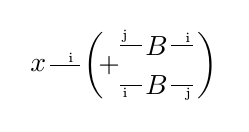
\begin{tikzpicture}[baseline=.5em, inner sep=1pt]
      \node (a0) at (0,0) {};
      \node (a1) at (.5,0) {$B$};
      \node (a2) at (1,0) {};
      \draw (a0) -- (a1) node[midway, below left, font=\tiny] {i};
      \draw (a1) -- (a2) node[midway, below right, font=\tiny] {j};
      \node (b0) at (0, .5) {};
      \node (b1) at (.5, .5) {$B$};
      \node (b2) at (1, .5) {};
      \draw (b0) -- (b1) node[midway, above left, font=\tiny] {j};
      \draw (b1) -- (b2) node[midway, above right, font=\tiny] {i};
      \node (l) at (-.3, .25) {$\bigg($};
      \node at (1.15, .25) {$\bigg)$};
      \node at (-.1, .25) {$+$};
      \node (x) at (-1,.25) {$x$};
      \draw (x) -- (l) node[midway, above right, font=\tiny] {i};
   \end{tikzpicture}
\end{walign}


TODO: Assume $W$ is symmetric, then... (84) - (88)

\subsection{Higher Order}
Integer powers of matrices, like $X^n$, are easy to handle by writing
out the product and using the product rule.
The Matrix Cookbook includes a few derivatives we can handle this way.
\begin{walign}
   \\[.5em]
   \tag{90}
   \frac{\partial\left(\mathbf{X}^n\right)_{k l}}{\partial X_{i j}}
   &=
  \sum_{r=0}^{n-1}\left(\mathbf{X}^r \mathbf{J}^{i j} \mathbf{X}^{n-1-r}\right)_{k l}
   &&
   \begin{tikzpicture}[baseline=(X0.base), inner sep=1pt]
      \node (X0) {$(X$};
      \node[right=.25 of X0] (X1) {$X$};
      \node[right=.25 of X1] (X2) {$X$};
      \node[right=.25 of X2] (X3) {$\dots$};
      \node[right=.25 of X3] (X4) {$X)$};
      \draw (X0) -- ++(-.5,0) node[midway, above left, font=\tiny] {k};
      \draw (X0) -- (X1) -- (X2) -- (X3) -- (X4);
      \draw (X4) -- ++(.5,0) node[midway, below right, font=\tiny] {l};
      \draw[d] (X4.east) -- ++(.2,.2)node[midway, above left, font=\tiny]{i};
      \draw[d] (X4.east) -- ++(.3,.1)node[midway, below right, font=\tiny]{j};
   \end{tikzpicture}
   \\
   &&&=\quad
   \begin{tikzpicture}[baseline=(X0.base), inner sep=1pt]
      \node (X0) {$(X)$};
      \node[right=.25 of X0] (X1) {$X$};
      \node[right=.25 of X1] (X2) {$X$};
      \node[right=.25 of X2] (X3) {$\dots$};
      \node[right=.25 of X3] (X4) {$X$};
      \draw (X0) -- ++(-.5,0) node[midway, above left, font=\tiny] {k};
      \draw (X0) -- (X1) -- (X2) -- (X3) -- (X4);
      \draw (X4) -- ++(.5,0) node[midway, below right, font=\tiny] {l};
      \draw[d] (X0.east) -- ++(.2,.2)node[midway, above left, font=\tiny]{i};
      \draw[d] (X0.east) -- ++(.3,.1)node[midway, below right, font=\tiny]{j};
   \end{tikzpicture}
 \\&&&+\quad\dots
 \\&&&+\quad
   \begin{tikzpicture}[baseline=(X0.base), inner sep=1pt]
      \node (X0) {$X$};
      \node[right=.25 of X0] (X1) {$X$};
      \node[right=.25 of X1] (X2) {$X$};
      \node[right=.25 of X2] (X3) {$\dots$};
      \node[right=.25 of X3] (X4) {$(X)$};
      \draw (X0) -- ++(-.5,0) node[midway, above left, font=\tiny] {k};
      \draw ++(-.5,0) -- (X0) -- (X1) -- (X2) -- (X3) -- (X4);
      \draw (X4) -- ++(.5,0) node[midway, below right, font=\tiny] {l};
      \draw[d] (X4.east) -- ++(.2,.2)node[midway, above left, font=\tiny]{i};
      \draw[d] (X4.east) -- ++(.3,.1)node[midway, below right, font=\tiny]{j};
   \end{tikzpicture}
 \\&&&=\quad
 \sum_{r=0}^{n-1}
   \begin{tikzpicture}[baseline=(X0.base), inner sep=1pt]
      \node (X0) {$X^r$};
      \node[right=.5 of X0] (X1) {$X^{n-r-1}$};
      \draw (X0.west) -- ++(-.25,0) node[midway, above left, font=\tiny] {k};
      \draw (X0.east) -- ++(.2,0) -- ++(.1,.2) node[midway, above left, font=\tiny] {i};
      \draw (X1.east) -- ++(.25,0) node[midway, below right, font=\tiny] {l};
      \draw (X1.west) -- ++(-.2,0) -- ++(-.1,-.2) node[midway, below right, font=\tiny] {j};
   \end{tikzpicture}
 \\
   \tag{91}
   \frac{\partial}{\partial \mathbf{X}} \mathbf{a}^T \mathbf{X}^n \mathbf{b}
   &=\sum_{r=0}^{n-1}\left(\mathbf{X}^r\right)^T \mathbf{a b}^T\left(\mathbf{X}^{n-1-r}\right)^T
   &&
   \begin{tikzpicture}[baseline=(X0.base), inner sep=1pt]
      \node (X0) {$(a-X$};
      \node[right=.25 of X0] (X3) {$\dots$};
      \node[right=.25 of X3] (X4) {$X-b)$};
      \draw (X0) -- (X3) -- (X4);
      \draw[d] (X4.east) -- ++(.2,.2);
      \draw[d] (X4.east) -- ++(.3,.1);
   \end{tikzpicture}
   \\
   &&&=\quad
   \sum_{r=0}^{n-1}
   \begin{tikzpicture}[baseline=(X0.base), inner sep=1pt]
      \node (X0) {$a-X^r$};
      \node[right=.5 of X0] (X1) {$X^{n-r-1}-b$};
      \draw (X0.east) -- ++(.25,.05) -- ++(-.1,.1);
      \draw (X1.west) -- ++(-.25,-.05) -- ++(.1,-.1);
   \end{tikzpicture}
   \\
   &&&=\quad
   \sum_{r=0}^{n-1}
   \begin{tikzpicture}[baseline=(X0.base), inner sep=1pt]
      \node (X0) {$-(X^r)^T-a$};
      \node[right=.25 of X0] (X1) {$b-(X^{n-r-1})^T-$};
   \end{tikzpicture}
\end{walign}


% Could be cool to do exponential here, if I could only find a good result for it...
% sum_{t>=1} 1/t! sum_{a+b=t-1} X^a X^b
% sum_{t>=1, a+b=t-1} X^a X^b / t!
% sum_{a>=0} sum_{b>=0} X^a X^b / (a+b+1)!


\section{Derivatives of Traces}
The Matrix Cookbook contains a lot of derivatives for traces.
These can be elegant in classical notation, since traces are scalar, so the derivatives are low order.

\subsection{First Order}

\begin{walign}
   \tag{99}
   \frac{\partial}{\partial X} \mathrm{Tr}(X)
   &= I
   &
   \hspace{-1em}
   \begin{tikzpicture}[baseline=(a0.base), inner sep=1pt]
      \node (a0) {$($};
      \node[right=1em of a0] (a1) {$X$};
      \node[right=1em of a1] (a3) {$)$};
      \path (a1) edge[out=160, in=20, loop] (a1);
      \draw[d] (a3.east) -- ++(.2,.2);
      \draw[d] (a3.east) -- ++(.3,.1);
   \end{tikzpicture}
   \hspace{-1em}
   &=
   \hspace{-2em}
   \begin{tikzpicture}[baseline=(a0.base), inner sep=1pt]
      \node (a1) {$(X)$};
      \path (a1) edge[out=160, in=20, loop, looseness=4] (a1);
      \draw[d] (a1.south east) -- ++(.2,-.2);
      \draw[d] (a1.south east) -- ++(.3,-.1);
   \end{tikzpicture}
   \hspace{-2em}
 \\&&&=
   \hspace{-1.5em}
   \begin{tikzpicture}[baseline=(a0.base), inner sep=1pt]
      \node (a1) {$\phantom{X}$};
      \path (a1) edge[out=160, in=20, loop, looseness=6] (a1);
      \draw ($(a1.east)-(0,-.2em)$) -- ++(.2,-.1);
      \draw ($(a1.west)-(0,-.2em)$) -- ++(-.2,-.1);
   \end{tikzpicture}
   \hspace{-1.5em}
 \\&&&=
   \matmul{\sbullet}
   %%%%%%%%%%%%%%%%%%%%%%%%%%%%%%
   \\
   \tag{100}
   \frac{\partial}{\partial X} \mathrm{Tr}(XA)
   &= A^T
   &
   \begin{tikzpicture}[baseline=(a0.base), inner sep=1pt]
      \node (a0) {$($};
      \node[right=1em of a0] (a1) {$X$};
      \node[right=1em of a1] (a2) {$A$};
      \node[right=1em of a2] (a3) {$)$};
      \draw (a1) -- (a2);
      \path (a1) edge[out=160, in=20, looseness=2] (a2);
      \draw[d] (a3.east) -- ++(.2,.2);
      \draw[d] (a3.east) -- ++(.3,.1);
   \end{tikzpicture}
   &=
   \hspace{-2em}
   \begin{tikzpicture}[baseline=(a0.base), inner sep=1pt]
      \node (a1) {$(X)$};
      \node[right=1em of a1] (a2) {$A$};
      \draw (a1) -- (a2);
      \path (a1) edge[out=160, in=20, looseness=2] (a2);
      \draw[d] (a1.south east) -- ++(.2,-.2);
      \draw[d] (a1.south east) -- ++(.3,-.1);
   \end{tikzpicture}
   \hspace{-2em}
 \\&&&=
   \hspace{-1.5em}
   \begin{tikzpicture}[baseline=(a0.base), inner sep=1pt]
      \node (a1) {$\phantom{X}$};
      \node[right=1em of a1] (a2) {$A$};
      \draw (a1) -- (a2);
      \path (a1) edge[out=160, in=20, looseness=2] (a2);
      \draw (a1.east) -- ++(.2,-.1);
      \draw ($(a1.west)-(0,-.2em)$) -- ++(-.2,-.1);
   \end{tikzpicture}
   \hspace{-1.5em}
 \\&&&
   = \matmul{A^T}
   %%%%%%%%%%%%%%%%%%%%%%%%%%%%%%
   \\
   \tag{101}
   \frac{\partial}{\partial X} \mathrm{Tr}(AXB)
   &= A^TB^T
   &
   \hspace{-1em}
   \begin{tikzpicture}[baseline=(a0.base), inner sep=1pt]
      \node (a0) {$($};
      \node[right=1em of a0] (a1) {$A$};
      \node[right=1em of a1] (a2) {$X$};
      \node[right=1em of a2] (a3) {$B$};
      \node[right=1em of a3] (a4) {$)$};
      \draw (a1) -- (a2) -- (a3);
      \path (a1) edge[out=160, in=20, looseness=1] (a3);
      \draw[d] (a4.east) -- ++(.2,.2);
      \draw[d] (a4.east) -- ++(.3,.1);
   \end{tikzpicture}
   &=
   \hspace{-1em}
   \begin{tikzpicture}[baseline=(a0.base), inner sep=1pt]
      \node (a1) {$A$};
      \node[right=1em of a1] (a2) {$(X)$};
      \node[right=1em of a2] (a3) {$B$};
      \draw (a1) -- (a2) -- (a3);
      \path (a1) edge[out=160, in=20, looseness=1] (a3);
      \draw[d] (a2.south east) -- ++(.2,-.2);
      \draw[d] (a2.south east) -- ++(.3,-.1);
   \end{tikzpicture}
 \\&&&=
   \hspace{-1em}
   \begin{tikzpicture}[baseline=(a0.base), inner sep=1pt]
      \node (a1) {$A$};
      \node[right=1em of a1] (a2) {$\phantom{X}$};
      \node[right=1em of a2] (a3) {$B$};
      \draw (a1) -- (a2) -- (a3);
      \path (a1) edge[out=160, in=20, looseness=1] (a3);
      \draw (a2.east) -- ++(.2,-.1);
      \draw (a2.west) -- ++(-.2,-.1);
   \end{tikzpicture}
 \\&&&=
   \matmul{A^T, B^T}
\end{walign}


Continues for (102-105).
The last one uses the Kronecker product, which we may have to introduce first.

\subsection{Second Order}
\begin{walign}
   \tag{106}
   \frac{\partial}{\partial X} \mathrm{Tr}(X^2)
   &=2 X^T
   &&
   \begin{tikzpicture}[baseline=(a0.base), inner sep=1pt]
      \node (a0) {$($};
      \node[right=.5em of a0] (a1) {$X$};
      \node[right=1em of a1] (a2) {$X$};
      \node[right=.5em of a2] (a3) {$)$};
      \draw (a1) -- (a2);
      \path (a1) edge[out=160, in=20, looseness=2] (a2);
      \draw[d] (a3.east) -- ++(.2,.2);
      \draw[d] (a3.east) -- ++(.3,.1);
   \end{tikzpicture}
 \\&&&=
   \hspace{-2em}
   \begin{tikzpicture}[baseline=(a0.base), inner sep=1pt]
      \node (a1) {$(X)$};
      \node[right=1em of a1] (a2) {$X$};
      \draw (a1) -- (a2);
      \path (a1) edge[out=160, in=20, looseness=2] (a2);
      \draw[d] (a1.south east) -- ++(.2,-.2);
      \draw[d] (a1.south east) -- ++(.3,-.1);
   \end{tikzpicture}
   \hspace{-2em}
   +
   \hspace{-2em}
   \begin{tikzpicture}[baseline=(a0.base), inner sep=1pt]
      \node (a1) {$X$};
      \node[right=1em of a1] (a2) {$(X)$};
      \draw (a1) -- (a2);
      \path (a1) edge[out=160, in=20, looseness=2] (a2);
      \draw[d] (a2.south east) -- ++(.2,-.2);
      \draw[d] (a2.south east) -- ++(.3,-.1);
   \end{tikzpicture}
   \hspace{-2em}
 \\&&&=
   \hspace{-1.5em}
   \begin{tikzpicture}[baseline=(a0.base), inner sep=1pt]
      \node (a1) {$\phantom{X}$};
      \node[right=1em of a1] (a2) {$X$};
      \draw (a1) -- (a2);
      \path (a1) edge[out=160, in=20, looseness=2] (a2);
      \draw (a1.east) -- ++(.2,-.1);
      \draw ($(a1.west)-(0,-.2em)$) -- ++(-.2,-.1);
   \end{tikzpicture}
   \hspace{-1.5em}
   +
   \hspace{-1.5em}
   \begin{tikzpicture}[baseline=(a0.base), inner sep=1pt]
      \node (a1) {$X$};
      \node[right=1em of a1] (a2) {$\phantom{X}$};
      \draw (a1) -- (a2);
      \path (a1) edge[out=160, in=20, looseness=2] (a2);
      \draw (a2.west) -- ++(-.2,-.1);
      \draw ($(a2.east)-(0,-.2em)$) -- ++(.2,-.1);
   \end{tikzpicture}
   \hspace{-1.5em}
 \\&&&=
   2\,\matmul{X^T}
   \\[1em]
   %%%%%%%%%%%%%%%%%%%%%%%%%%%%%%%%%%%%%%%%%%%%%%%%%%%%%%%%%%%%%%%%%%%%%%%%%%%%%%%%
   \tag{107}
   \frac{\partial}{\partial X} \mathrm{Tr}(X^2 B)
   &=(XB+BX)^T
   &&
   \begin{tikzpicture}[baseline=(a0.base), inner sep=1pt]
      \node (a0) {$($};
      \node[right=.5em of a0] (a1) {$X$};
      \node[right=1em of a1] (a2) {$X$};
      \node[right=1em of a2] (a3) {$B$};
      \node[right=.5em of a3] (a4) {$)$};
      \draw (a1) -- (a2) -- (a3);
      \path (a1) edge[out=160, in=20, looseness=1] (a3);
      \draw[d] (a4.east) -- ++(.2,.2);
      \draw[d] (a4.east) -- ++(.3,.1);
   \end{tikzpicture}
  \\&&&=
   \hspace{-1.5em}
   \begin{tikzpicture}[baseline=(a0.base), inner sep=1pt]
      \node (a1) {$(X)$};
      \node[right=1em of a1] (a2) {$X$};
      \node[right=1em of a2] (a3) {$B$};
      \draw (a1) -- (a2) -- (a3);
      \path (a1) edge[out=160, in=20, looseness=1] (a3);
      \draw[d] (a1.south east) -- ++(.2,-.2);
      \draw[d] (a1.south east) -- ++(.3,-.1);
   \end{tikzpicture}
   \hspace{-1.5em}
   +
   \hspace{-1.5em}
   \begin{tikzpicture}[baseline=(a0.base), inner sep=1pt]
      \node (a1) {$X$};
      \node[right=1em of a1] (a2) {$(X)$};
      \node[right=1em of a2] (a3) {$B$};
      \draw (a1) -- (a2) -- (a3);
      \path (a1) edge[out=160, in=20, looseness=1] (a3);
      \draw[d] (a2.south east) -- ++(.2,-.2);
      \draw[d] (a2.south east) -- ++(.3,-.1);
   \end{tikzpicture}
   \hspace{-1.5em}
 \\&&&=
   \hspace{-1.5em}
   \begin{tikzpicture}[baseline=(a0.base), inner sep=1pt]
      \node (a1) {$\phantom{X}$};
      \node[right=1em of a1] (a2) {$X$};
      \node[right=1em of a2] (a3) {$B$};
      \draw (a1) -- (a2) -- (a3);
      \path (a1) edge[out=160, in=20, looseness=1] (a3);
      \draw (a1.east) -- ++(.2,-.1);
      \draw ($(a1.west)-(0,-.2em)$) -- ++(-.2,-.1);
   \end{tikzpicture}
   \hspace{-1.5em}
   +
   \hspace{-1.5em}
   \begin{tikzpicture}[baseline=(a0.base), inner sep=1pt]
      \node (a1) {$X$};
      \node[right=1em of a1] (a2) {$\phantom{X}$};
      \node[right=1em of a2] (a3) {$B$};
      \draw (a1) -- (a2) -- (a3);
      \path (a1) edge[out=160, in=20, looseness=1] (a3);
      \draw (a2.west) -- ++(-.2,-.1);
      \draw (a2.east) -- ++(.2,-.1);
   \end{tikzpicture}
   \hspace{-1.5em}
 \\&&&=
   \matmul{B^T, X^T}
   + \matmul{X^T, B^T}
   \\[1em]
%%%%%%%%%%%%%%%%%%%%%%%%%%%%%%%%%%%%%%%%%%%%%%%%%%%%%%%%%%%%%%%%%%%%%%%%%%%%%%%%
   \tag{108, 109, 110}
   \frac{\partial}{\partial X} \mathrm{Tr}(X^T B X)
    &=
   \frac{\partial}{\partial X} \mathrm{Tr}(X X^T B)
    &&
   \begin{tikzpicture}[baseline=(a0.base), inner sep=1pt]
      \node (a0) {$($};
      \node[right=.5em of a0] (a1) {$X^T$};
      \node[right=1em of a1] (a2) {$B$};
      \node[right=1em of a2] (a3) {$X$};
      \node[right=.5em of a3] (a4) {$)$};
      \draw (a1) -- (a2) -- (a3);
      \path (a1) edge[out=160, in=20, looseness=1] (a3);
      \draw[d] (a4.east) -- ++(.2,.2);
      \draw[d] (a4.east) -- ++(.3,.1);
   \end{tikzpicture}
 \\&
   =\frac{\partial}{\partial X} \mathrm{Tr}(B X X^T)
   &&=
   \hspace{-2em}
   \begin{tikzpicture}[baseline=(a0.base), inner sep=1pt]
      \node (a1) {$(X^T)$};
      \node[right=1em of a1] (a2) {$B$};
      \node[right=1em of a2] (a3) {$X$};
      \draw (a1) -- (a2) -- (a3);
      \path (a1) edge[out=160, in=20, looseness=1] (a3);
      \draw[d] (a1.south east) -- ++(.2,-.2);
      \draw[d] (a1.south east) -- ++(.3,-.1);
   \end{tikzpicture}
   \hspace{-2em}
   +
   \hspace{-2em}
   \begin{tikzpicture}[baseline=(a0.base), inner sep=1pt]
      \node (a1) {$X^T$};
      \node[right=1em of a1] (a2) {$B$};
      \node[right=1em of a2] (a3) {$(X)$};
      \draw (a1) -- (a2) -- (a3);
      \path (a1) edge[out=160, in=20, looseness=1] (a3);
      \draw[d] (a3.south east) -- ++(.2,-.2);
      \draw[d] (a3.south east) -- ++(.3,-.1);
   \end{tikzpicture}
 \\&
   =(B+B^T)X
   &&=
   \hspace{-1.5em}
   \begin{tikzpicture}[baseline=(a0.base), inner sep=1pt]
      \node (a1) {$\phantom{X}$};
      \node[right=1em of a1] (a2) {$B$};
      \node[right=1em of a2] (a3) {$X$};
      \draw (a1) -- (a2) -- (a3);
      \path (a1) edge[out=160, in=20, looseness=1] (a3);
      \draw ($(a1.west)-(0,-.2em)$) -- ++(.1,-.05);
   \end{tikzpicture}
   \hspace{-1.5em}
   +
   \hspace{-1.5em}
   \begin{tikzpicture}[baseline=(a0.base), inner sep=1pt]
      \node (a1) {$X^T$};
      \node[right=1em of a1] (a2) {$B$};
      \node[right=1em of a2] (a3) {$\phantom{X}$};
      \draw (a1) -- (a2) -- (a3);
      \path (a1) edge[out=160, in=20, looseness=1] (a3);
      \draw (a3.west) -- ++(-.2,-.1);
      \draw ($(a3.east)-(0,-.2em)$) -- ++(.2,-.1);
   \end{tikzpicture}
   \\
   &&&=
   \matmul{B, X}
   + \matmul{B^T, X}
   \\[1em]
   \tag{111, 112, 113}
%%%%%%%%%%%%%%%%%%%%%%%%%%%%%%%%%%%%%%%%%%%%%%%%%%%%%%%%%%%%%%%%%%%%%%%%%%%%%%%%
   \frac{\partial}{\partial X} \mathrm{Tr}(X B X^T)
    &=
   \frac{\partial}{\partial X} \mathrm{Tr}(X^T X B)
    &&
   \begin{tikzpicture}[baseline=(a0.base), inner sep=1pt]
      \node (a0) {$($};
      \node[right=.5em of a0] (a1) {$X$};
      \node[right=1em of a1] (a2) {$B$};
      \node[right=1em of a2] (a3) {$X^T$};
      \node[right=.5em of a3] (a4) {$)$};
      \draw (a1) -- (a2) -- (a3);
      \path (a1) edge[out=160, in=20, looseness=1] (a3);
      \draw[d] (a4.east) -- ++(.2,.2);
      \draw[d] (a4.east) -- ++(.3,.1);
   \end{tikzpicture}
 \\&
   =\frac{\partial}{\partial X} \mathrm{Tr}(B X^T X)
   &&=
   \hspace{-2em}
   \begin{tikzpicture}[baseline=(a0.base), inner sep=1pt]
      \node (a1) {$(X)$};
      \node[right=1em of a1] (a2) {$B$};
      \node[right=1em of a2] (a3) {$X^T$};
      \draw (a1) -- (a2) -- (a3);
      \path (a1) edge[out=160, in=20, looseness=1] (a3);
      \draw[d] (a1.south east) -- ++(.2,-.2);
      \draw[d] (a1.south east) -- ++(.3,-.1);
   \end{tikzpicture}
   \hspace{-2em}
   +
   \hspace{-2em}
   \begin{tikzpicture}[baseline=(a0.base), inner sep=1pt]
      \node (a1) {$X$};
      \node[right=1em of a1] (a2) {$B$};
      \node[right=1em of a2] (a3) {$(X^T)$};
      \draw (a1) -- (a2) -- (a3);
      \path (a1) edge[out=160, in=20, looseness=1] (a3);
      \draw[d] (a3.south east) -- ++(.2,-.2);
      \draw[d] (a3.south east) -- ++(.3,-.1);
   \end{tikzpicture}
 \\&
   =X(B^T+B)
   &&=
   \hspace{-1.5em}
   \begin{tikzpicture}[baseline=(a0.base), inner sep=1pt]
      \node (a1) {$\phantom{X}$};
      \node[right=1em of a1] (a2) {$B$};
      \node[right=1em of a2] (a3) {$X^T$};
      \draw (a1) -- (a2) -- (a3);
      \path (a1) edge[out=160, in=20, looseness=1] (a3);
      \draw (a1.east) -- ++(.2,-.1);
      \draw ($(a1.west)-(0,-.2em)$) -- ++(-.2,-.1);
   \end{tikzpicture}
   \hspace{-1.5em}
   +
   \hspace{-1.5em}
   \begin{tikzpicture}[baseline=(a0.base), inner sep=1pt]
      \node (a1) {$X$};
      \node[right=1em of a1] (a2) {$B$};
      \node[right=1em of a2] (a3) {$\phantom{X}$};
      \draw (a1) -- (a2) -- (a3);
      \path (a1) edge[out=160, in=20, looseness=1] (a3);
   \end{tikzpicture}
   \\
   &&&=
   \matmul{X, B^T} + \matmul{X, B}
\end{walign}

The last equation is a bit surprising, since we might assume
we could simply substitute $X$ for $X^T$ in the previous equation
and conclude
\[
   (B+B^T)X
   =
   \frac{\partial}{\partial X} \mathrm{Tr}(X B X^T)
   =
   \frac{\partial}{\partial X} \mathrm{Tr}(X^T B X)
   = X(B^T + B).
\]
However that is clearly not that case.
Such substitution would only work for a linear function, not a quadratic.
In general it is the case that
$\frac{\partial}{\partial X} f(X)^T \neq
\frac{\partial}{\partial X} f(X^T)$.
%Instead we have
%\[
%   \frac{\partial}{\partial X} \mathrm{Tr}(X B X^T)
%   = \frac{\partial}{\partial X} \mathrm{Tr}((X B X^T)^T)
%   = \frac{\partial}{\partial X} \mathrm{Tr}(X B^T X^T)
%\]

\subsection{Higher Order}



\begin{walign}
   \tag{121}
   \frac{\partial}{\partial X}\mathrm{Tr}(X^n)
   &=
   n(X^{n-1})^T
   &&
   \begin{tikzpicture}[baseline=(X0.base), inner sep=1pt]
      \node (X0) {$(X$};
      \node[right=.25 of X0] (X1) {$X$};
      \node[right=.25 of X1] (X2) {$X$};
      \node[right=.25 of X2] (X3) {$\dots$};
      \node[right=.25 of X3] (X4) {$X)$};
      \draw (X0) -- (X1) -- (X2) -- (X3) -- (X4);
      \path (X0) edge[out=160, in=20, looseness=1] (X4);
      \draw[d] (X4.south east) -- ++(.2,-.2);
      \draw[d] (X4.south east) -- ++(.3,-.1);
   \end{tikzpicture}
   \\
   &&&=\quad
 \sum_{r=0}^{n-1}
   \hspace{-1.5em}
   \begin{tikzpicture}[baseline=(X0.base), inner sep=1pt]
      \node (X0) {$X^r$};
      \node[right=.5 of X0] (X1) {$X^{n-r-1}$};
      \draw (X0.east) -- ++(.25,.05) -- ++(-.1,.1);
      \draw (X1.west) -- ++(-.25,-.05) -- ++(.1,-.1);
      \path (X0) edge[out=160, in=20, looseness=1] (X1);
   \end{tikzpicture}
   \\
   &&&=\quad
   n
   (X^T)^{n-1}
%%%%%%%%%%%%%%%%%%%%%%%%%%%%%%%%%%%%%%%%%%%%%%%%%%%%%%%%%%%%%%%%%%%%%%%%%%%%%%%%
   \\[1em]
   \tag{122}
   \frac{\partial}{\partial X} \mathrm{Tr}(AX^n)
   &=\sum_{r=0}^{n-1}(X^r A X^{n-1-r})^T
   &&
   \begin{tikzpicture}[baseline=(X0.base), inner sep=1pt]
      \node (X0) {$(A$};
      \node[right=.25 of X0] (X1) {$X$};
      \node[right=.25 of X1] (X2) {$X$};
      \node[right=.25 of X2] (X3) {$\dots$};
      \node[right=.25 of X3] (X4) {$X)$};
      \draw (X0) -- (X1) -- (X2) -- (X3) -- (X4);
      \path (X0) edge[out=160, in=20, looseness=1] (X4);
      \draw[d] (X4.south east) -- ++(.2,-.2);
      \draw[d] (X4.south east) -- ++(.3,-.1);
   \end{tikzpicture}
   \\
   &&&=\quad
   \sum_{r=0}^{n-1}
   \hspace{-2em}
   \begin{tikzpicture}[baseline=(X0.base), inner sep=1pt]
      \node (A) {$A$};
      \node[right=.25 of A] (X0) {$X^r$};
      \node[right=.5 of X0] (X1) {$X^{n-r-1}$};
      \draw (X0.east) -- ++(.25,.05) -- ++(-.1,.1);
      \draw (X1.west) -- ++(-.25,-.05) -- ++(.1,-.1);
      \draw (A) -- (X0);
      \path (A) edge[out=160, in=20, looseness=1] (X1);
   \end{tikzpicture}
   \\
   &&&=\quad
   \sum_{r=0}^{n-1}
   \matmul{(X^r)^T, A^T, (X^{n-r-1})^T}
\end{walign}


\section{Exercises}
\begin{exercise}
   Find the derivative of \[x^T A^T x x^T A x\] with respect to $x$.
\end{exercise}

\begin{exercise}
   Find the derivative of \[X^T A X\] with respect to $X$.
\end{exercise}

\begin{exercise}
   Show the derivatives:
   \begin{align*}
   \tag{78}
   \frac{\partial}{\partial x} (Bx+b)^T C (Dx+d)
   &= B^TC(Dx+d) + D^TC^T(Bx+b)
   \\
   \tag{82}
   \frac{\partial}{\partial X} b^T X^T D X c
   &= D^T X b c^T + DXcb^T
   \\
   \tag{83}
   \frac{\partial}{\partial X} (Xb+c)^T D (Xb+c)
   &= (D+D^T)(Xb+c)b^T
   \end{align*}
\end{exercise}

\begin{exercise}
   Show the remaining second order trace derivatives from the Matrix Cookbook:
   \begin{align*}
      \tag{114}
   \frac{\partial}{\partial X} \operatorname{Tr}(A X B X)
   &=A^T X^T B^T+B^T X^T A^T
   \\
   \tag{115}
   \frac{\partial}{\partial X} \operatorname{Tr}\left(X^T X\right)
   &=\frac{\partial}{\partial X} \operatorname{Tr}\left(X X^T\right)=2 X
   \\
   \tag{116}
   \frac{\partial}{\partial X} \operatorname{Tr}\left(B^T X^T C X B\right)
   &=C^T X B B^T+C X B B^T
   \\
   \tag{117}
   \frac{\partial}{\partial X} \operatorname{Tr}\left[X^T B X C\right]
   &=B X C+B^T X C^T
   \\
   \tag{118}
   \frac{\partial}{\partial X} \operatorname{Tr}\left(A X B X^T C\right)
   &=A^T C^T X B^T+C A X B
   \\
   \tag{119}
   \frac{\partial}{\partial X} \operatorname{Tr}\left[(A X B+C)(A X B+C)^T\right]
   &=2 A^T(A X B+C) B^T
   \\
   \end{align*}
\end{exercise}

\begin{exercise}
   Show the derivative of the fourth order trace from the Matrix Cookbook:
   \begin{align*}
      \tag{123}
\frac{\partial}{\partial X} \operatorname{Tr}\left[B^T X^T C X X^T C X B\right]
&= C X X^T C X B B^T 
\\&+ C^T X B B^T X^T C^T X 
\\&+ C X B B^T X^T C X 
\\&+ C^T X X^T C^T X B B^T
   \end{align*}
\end{exercise}
